\documentclass{report}
\usepackage[utf8]{inputenc}
\usepackage[english]{duomasterforside}
\usepackage{graphicx}
\usepackage{caption}
\usepackage{subcaption}
\usepackage{hyperref}
\setcounter{secnumdepth}{1}
\setcounter{tocdepth}{3}
\begin{document}
\title{Master's Essay}
\duoforside[author={Adrian Eriksen}, dept={Department of Informatics}, program={Language Technology}]

\tableofcontents
\newpage
\chapter{Background}
\section{Introduction}
In this essay I will explain the challenges of cross-domain sentiment analysis and how we might use transfer learning to solve it.
Sentiment analysis is the process of trying to understand the sentiment behind a statement or document using machine learning. This can, among other things, be used to get information from reviews that can provide useful information.
There are many different ways to formulate a sentiment. A movie review might state "The movie is not bad at all.". If we simply look for words like "bad" and classify them as negative, we will get inaccurate results.\\\\
First, I will explain some of the technologies that has created the foundation for what we now use in language technology.
\\\\  - Structure of essay - \\\\
Pretraining:\\ 
BERT\\
ELMO\\
task specific\\

%Number sections

\newpage


\section{Sentiment Analysis}
Sentiment analysis (SA) is the computational treatment of opinions, sentiments, and subjectivity of texts. SA is also known as opinion mining and a few other terms and has a variety of different applications. It can be used for labeling reviews of movies or books, opinion mining from sites like Twitter.\\\\% and determining whether a written text is casual, informative, or friendly, like Grammarly.
SA can be done on different levels of text. Document-level SA is the task of classifying the sentiment of a document. The document in this context will be considered as one piece of information, and the score this document receives is determined by the overall sentiment of the author. By applying SA to different documents regarding the same topic, we get a score based on the total number of positive and negative documents.\\
Sentence-level SA looks at each sentence as positive, negative, or neutral, sometimes with different intensities. When looking at the sentences in a document, there are different levels of subjectivity that can be observed. Some sentences will only state a fact like "The restaurant serves Italian food", while others contain subjective opinions like "The restaurant closes too early". The subjectivity of sentences can affect the intensity, as a sentence based on an opinion or a certain belief, usually indicates a stronger intensity than stating a fact.\\%
%Talk about fine-grained in general and aspect based is a subset
Aspect-based SA is different than the two other approaches. Instead of trying to classify a word, sentence, or document as either positive or negative, aspect-based SA is tasked with identifying different aspects associated with a target \cite{pontiki-etal-2016-semeval}. One of the main contributions of aspect-based SA is that in addition to learning whether a review is positive or negative, you also learn which aspects of the review that made it so. If we're looking at a review for a hotel, we could retrieve information like "The breakfast was good", "They never made our bed". With information like this, we can assign the aspect, food, of the target, hotel, has a positive polarity. Likewise, the aspect, service - room, of the target, hotel, has a negative polarity. Being able to extract features like this instead of just "The hotel got a score of 3", is very valuable to most businesses since many consumers share their experiences with products online.\\\\
As of today, there are two main approaches to SA, the lexicon-based approach and the machine learning approach. The lexicon-based approach is mostly used on a document-level or sentence-level and uses a lexicon with words or multiword terms. These are usually tagged with sentiment (positive or negative) and sometimes with different intensities (very positive, slightly negative, etc). Given the word or multiword terms, you can further calculate the value of a sentence and then the entire document. One way to do this is by assigning each word a score with either positive or negative numbers while taking negation into account. For example, "The movie was not excellent" should yield a higher score than "The movie was not good", as a strongly polarized word usually reflects a somewhat mixed opinion \cite{taboada-etal-2011-lexicon}. One of the benefits of lexicon-based SA is that you don't have any need for labeled data, as the lexicon is pre-defined, and that you get some robustness when applying it on different domains if the lexicon is well made \cite{taboada-etal-2011-lexicon}.\\
The machine learning approach can create a model from a labeled training dataset and then apply it to the target data through standard machine learning methods \cite{pang-etal-2002-thumbs}, vectorization \cite{Peters:2018, mikolov2013efficient, pennington2014glove} or use a premade model and fine-tuning it on the target data \cite{DBLP:journals/corr/abs-1810-04805}. The aforementioned machine learning approaches use unsupervised, semi-supervised and supervised learning. What they all have in common, is that they don't reference any lexicon with pre-defined sentiments. You train an algorithm on graded reviews, and then have it predict the grade given to unseen reviews. Much like the lexicon-based approach, machine learning can be done on both document-level and sentence-level SA.\\
One final approach that has been used for all granularities of SA is a hybrid between the machine learning and lexicon-based approach \cite{zhang2011combining}, where you first train an algorithm on labeled data, before comparing the results with a lexicon to improve accuracy. This approach can also be used for aspect-based SA \cite{brun2016xrce}.
One of the original challenges with SA was that sentiment is rarely identifiable by keywords alone \cite{pang-etal-2002-thumbs}. When humans are presented with the task of selecting a set of keywords to tell whether a movie review is positive or negative, our intuition often leads us towards words like "horrible", "boring" and "sucks" for negative reviews, and "excellent", "thrilling" and "amazing" for positive reviews. As it turns out, selecting words like these gives us a much lower accuracy than if we train a model on labeled reviews, letting the model figure out which words are important. 
\\


%Some of the early work on SA focus explicitly on subjective sentences
%What is problematic with sentence level? Mixed polarity, 
%Done?:
%Domain effects for SA
%Talk about lexicon vs other methods
%Mention different granularities word/sentence/intensities just mention variations (include that it can be used on different levels, SA for a single sentence for example)

\section{Datasets}
%In NLP most data is in English, in this section I will discuss some of the most used datasets, which are all in English
There is a lot of different datasets that are commonly used for sentiment analysis, covering a variety of domains. The dataset that I will use is in Norwegian, but most of the data used in NLP is in English. In this section, I will discuss some of the most common English ones, before taking a closer look at the one I will use.
\subsection{Stanford Sentiment Treebank}
The Standford Sentiment Treebank \cite{socher2013recursive} is a dataset consisting of 11.855 single sentences from movie reviews and fine-grained sentiment labels for 215 thousand phrases. The sentiments are rated between 1 and 25, which makes the annotations very detailed. The dataset has been used as a benchmark to test new language models, as a way to demonstrate high performance.
\subsection{IMDb Movie Review Dataset}
The IMDb Movie Review Dataset \cite{maas-EtAl:2011:ACL-HLT2011} has close to 50.000 movie reviews, with 25.000 being labeled as positive and 25.000 as negative. It's a dataset for binary sentiment classification, where there are no more than 30 reviews for any given movie. The dataset contains reviews with a score equal to or below 4/10, or a score equal to or above 7/10 so that there are no neutral ratings.
\subsection{Amazon Review Data}
Amazon Review Data \cite{ni2019justifying} is a dataset containing 233.1 million product reviews and metadata from Amazon. It includes reviews consisting of text, ratings and helpfulness votes, product metadata consisting of descriptions, category information, price, brand and image features, and links to "also viewed/also bought graphs. The reviews cover 29 different domains including books, music, electronics, video games, beauty, and toys, albeit all of them are Amazon-products.
\subsection{Twitter}
Twitter has long been one of the most important and influential data-source for opinion mining. Already back in 2010, it had millions of users tweeting daily, sharing their opinion on almost everything \cite{pak-paroubek-2010-twitter}. The use of hashtags makes the data more easily separable, the word-limit per tweet makes each document concise, and the amount of data grows every day.
%To do:
%What has been done for SA in Norwegian?

%NoReC
%In contrast it's a multidomain dataset

\subsection{NoReC}
The Norwegian Review Corpus (NoReC) is a dataset containing more than 35,000 full-text reviews from Norwegian news sources \cite{VelOvrBer18}.\\
NoReC covers a range of different domains, including literature, movies, video games, restaurants, music, and theater, in addition to product reviews across a range of categories. Each review is labeled with a score ranging from 1-6, provided by the author of the review. NoReC was primarily created for training and evaluating models for document-level sentiment analysis, which makes it ideal for testing differences between domains on a document-level. The dataset has a good spread between scores, with 3, 4, and 5 being the most frequent. This makes sense, as it usually takes something particularly bad to give a score of 1 or 2, or something extraordinary to give a score of 6. Figure \ref{fig:ratings} shows a distribution of the ratings. Looking at the distributions of the categories, we can see from figure \ref{fig:cat_dist} that the categories 'screen' and 'music' is the most represented by far. One of the reasons for this is that the different sources label their categories differently. Upon further inspection, we can see from figure \ref{fig:screen} and figure \ref{fig:music} that these actually cover a variety of different categories from the different sources (I have removed the categories 'utenriks', 'kjendis' and 'nyheter' from figure \ref{fig:screen} because these represented one, four and one reviews respectively).

%Distribution of domains
%Get more specific numbers
%Transition into domain adaptation
%Set up tables with counts etc
%Get more statistics
%Mention NoReC_fine
\begin{figure}[h!]
	\centering
	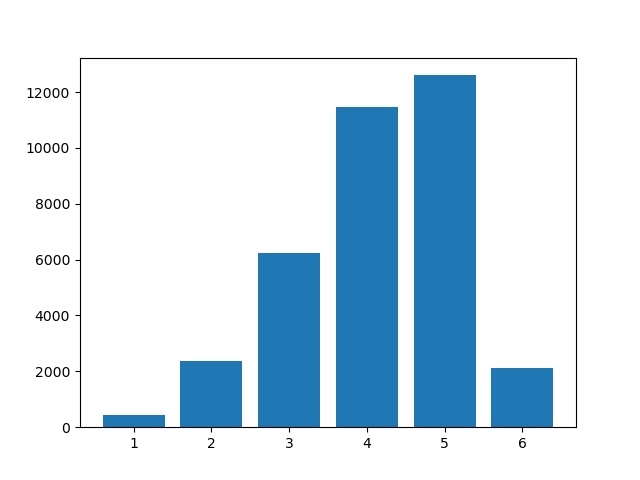
\includegraphics[scale=0.5]{img/ratings}
	\caption{Distribution of ratings in the NoReC dataset}
	\label{fig:ratings}
\end{figure}%
\begin{figure}[h!]
		\centering
		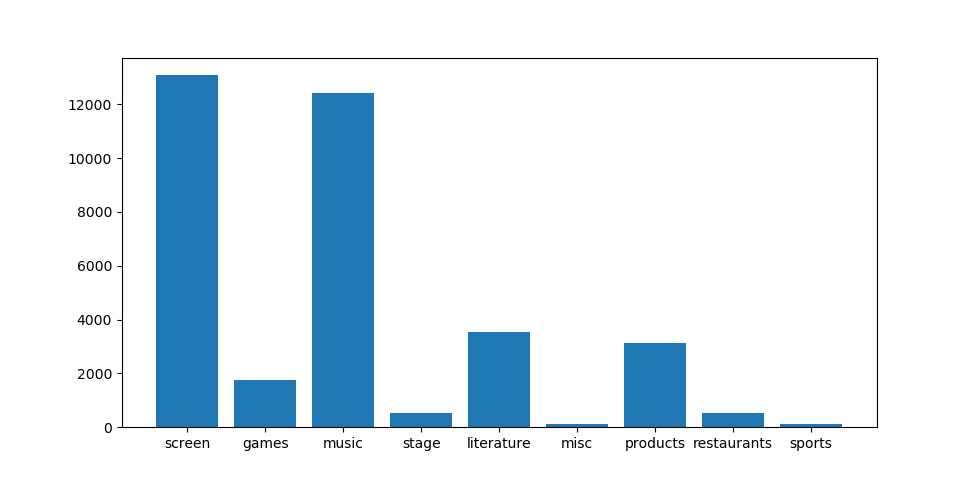
\includegraphics[scale=0.5]{img/cat_dist}
		\caption{The distribution of categories in the NoReC dataset}
		\label{fig:cat_dist}
	\end{figure}%
\begin{figure}[h!]
		\centering
		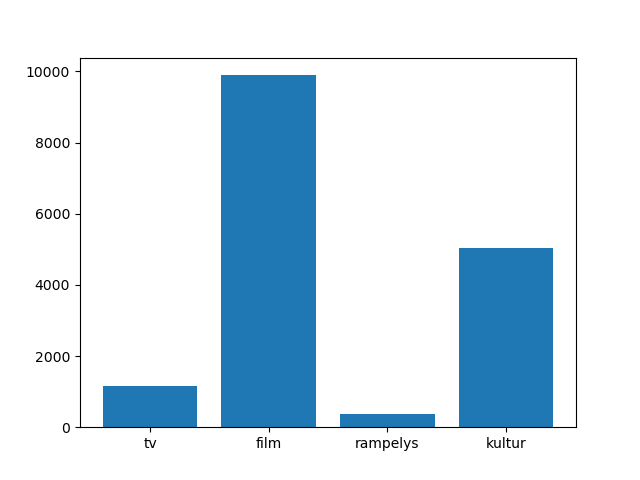
\includegraphics[scale=0.5]{img/screen_categories}
		\caption{The different categories found under 'screen'}
		\label{fig:screen}
\end{figure}%
\begin{figure}[h!]
	\centering
	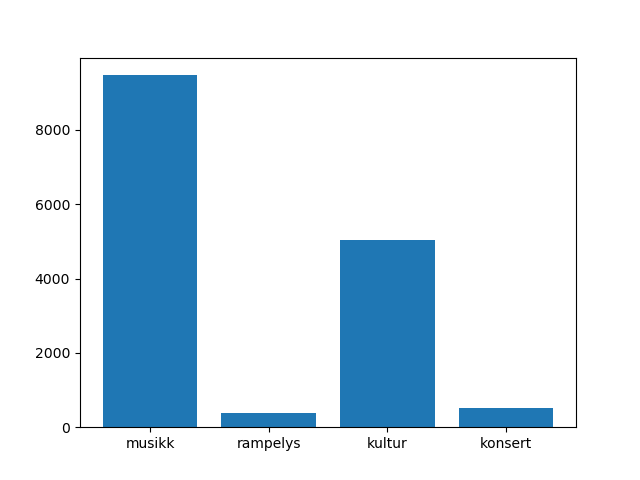
\includegraphics[scale=0.5]{img/music_categories}
	\caption{The different categories found under 'music'}
	\label{fig:music}
\end{figure}%
\begin{figure}[h!]
	\centering
	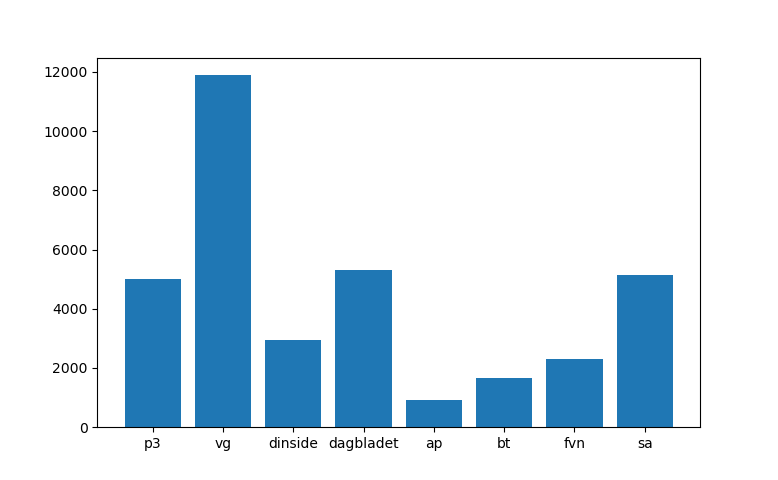
\includegraphics[scale=0.5]{img/src_dist}
	\caption{The different sources in the NoReC dataset}
	\label{fig:sources}
\end{figure}%

% -> Domain Adaptation
\section{Domain Adaptation}
Domain adaptation is the task of developing learning algorithms that takes knowledge from labeled data in a source domain and adapt the knowledge to different domains. This is especially interesting in NLP, as we often have a large amount of labeled data in a source domain (e.g IMDb Movie Review Dataset). The prospect of applying the knowledge from an algorithm trained on one domain, to another where we have little to none labeled data, is very appealing. This raises a challenge, however. If we train a model on a specific domain (e.g movie reviews), it transfers poorly to other domains like restaurant reviews. In the movie review domain, some of the words that carries negative weight is words like "2", "series" and "tv", which makes sense in that specific domain (people tend to disfavor movies based on tv series, and sequels). However, for the restaurant domain, the opposite might be true. If a restaurant has been on tv, or is part of a series, it might be a positive thing. This creates a challenge when we train a model on a specific domain and try to apply it to another.

% -> Transfer Learning
\subsection{Transfer Learning}
Transfer learning is a means to extract knowledge from a source setting and apply it to a different target setting. If you have a source domain $D_S$ and learning task $T_S$, a target domain $D_T$ and learning task $T_T$, transfer learning aims to improve the performance on $D_T$ using knowledge from $D_S$ and $T_S$ \cite{5288526}. According to Pan and Yang, there are three main research issues in transfer learning: 1) what to transfer, 2) how to transfer, and 3) when to transfer. What to transfer, is the task of finding the information that is relevant as well as irrelevant to transfer between the domains. Secondly, we must develop an algorithm that can transfer the information in a satisfactory manner, which is how to transfer. When to transfer is the task of knowing when transfer learning is helpful, and when it's disruptive. Using transfer learning on two completely separate domains may hurt the model's performance\cite{5288526}.\\
There are a variety of different types within transfer learning. A taxonomy that shows the variations can be seen in \ref{fig:tltax}.
\begin{figure}[h!]
	\centering
	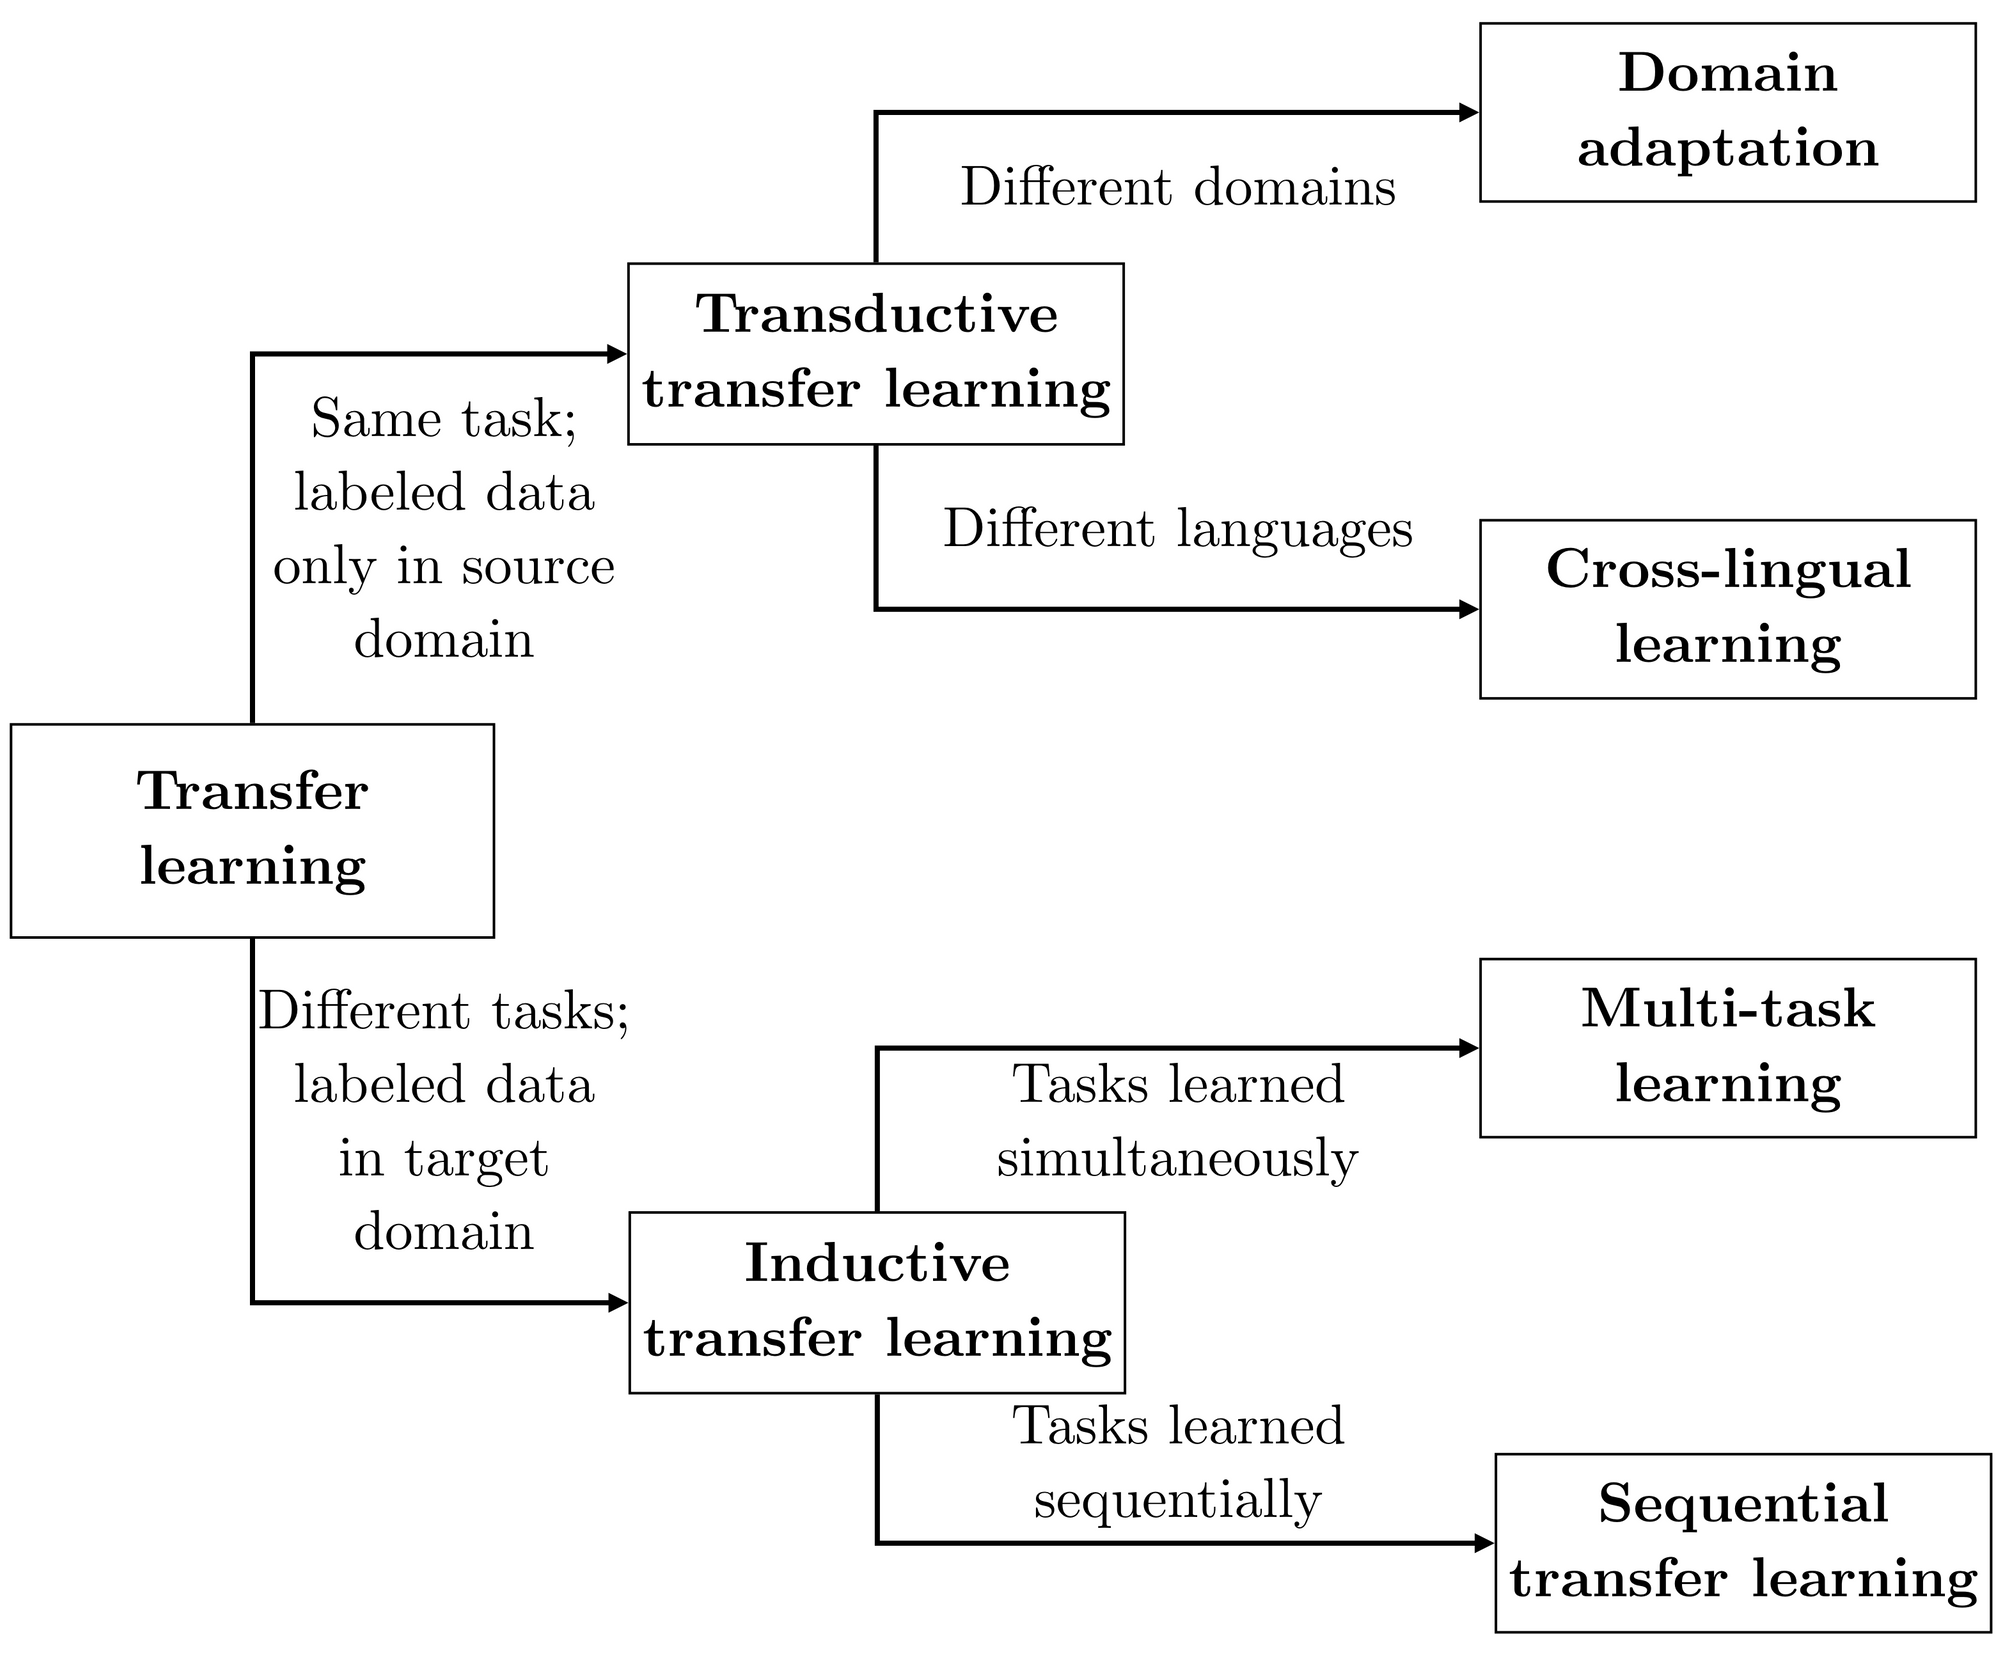
\includegraphics[scale=0.13]{img/tl_taxonomy}
	\caption{A taxonomy for transfer learning in NLP \href{ruder.io/thesis/neural_transfer_learning_for_nlp.pdf}{Ruder, 2019}}
		\label{fig:tltax}
\end{figure}%
In NLP this can be especially useful because words often mean the same in a given context. There are, however, a few different types of transfer learning. One is when you have labeled data in the source domain and adapt the knowledge to different domains, also known as domain adaptation. A different, more common approach, is training on a large amount of unlabeled data, before adapting the representations using self-supervised learning.

\subsection{Pre-Training}
\noindent
%Talk about word embeddings and vectors as examples, but don't explain them
%Word2Vec
Pre-training in NLP is the task of modeling complex characteristics of word use, and apply this model on several different tasks.
Pre-training is usually done on large amounts of data and has in recent years been used to produce word embeddings. Without going into too much detail, word embeddings aims to capture contexts of words, like "king is to queen as man is to woman". The most commonly used word embeddings can be divided into static and contextualized embeddings. I will first do a short explanation of static embeddings, before discussing contextualized embeddings and finetuning in more detail.

\subsection{Static Embeddings}
Static word embeddings had a breakthrough when Google published their Word2Vec algorithm in 2013 \cite{mikolov2013efficient}. This was a breakthrough in NLP, as we now had access to over 1.4 million vectors trained on more than 100 billion words. Word2Vec could be implemented using two different approaches. The first is the continuous bag of words (CBOW), where we try to predict which word is most likely given its context. The second is skip-gram, where we try to predict the context from a word. About a year later, Stanford published their version of static word embeddings called GloVe \cite{pennington2014glove}. In short, what GloVe did differently was that it focused on co-occurrences of words, looking at the probabilities that two words appear together.

%contextualized embeddings - computing vectors in context instead of fixed
%can also be trained from scartch, but they are more commonly pretrained
%can be fine-tuned or used as is -> Domain Adaptation
%finetuning can be used for domain adaptation
\subsection{Contextualized Embeddings}
Contextualized embeddings were the next step in pre-training language models. In 2018, Embeddings from Language Models (ELMo) was published \cite{Peters:2018}. Where we previously assigned a vector to each word, ELMo looks at the context the word appears in. If we take the word "fall", this could have multiple meanings. One being the verb "to fall", another being the time of year as in "autumn". With traditional embeddings, we would learn the vectors based on a dataset and assign only one vector to "fall". One of the revolutionary things that ELMo did, is that each token is assigned a representation that is a function of the entire input sentence. In other words, the embedding assigned to "fall" is calculated from the sentence it appears in. The way ELMo does this is by using a bidirectional long short-term memory (BiLSTM) RNN to calculate the probability of both previous and future words in the sentence, before returning the contextualized embedding.\\
Not long after the release of ELMO, Bidirectional Encoder Representations from Transformers (BERT) was published \cite{DBLP:journals/corr/abs-1810-04805}. Upon its release in 2018, it obtained state-of-the-art results on eleven NLP tasks in a variety of fields, using Google's transformer architecture \cite{DBLP:journals/corr/VaswaniSPUJGKP17}. Whereas previous language representation models using transformers had been unidirectional \cite{radford2018improving}, BERT uses attention mechanisms to learn the contextual relations between all words in a sentence. The way BERT does this is by using a "masked language model" (MLM) pre-training objective. First, the model replaces some of the words in the dataset with the [MASK] token, then the model attempts to predict the actual value of the token, based on the context provided by the unmasked words in the sentence. Next, the model does "next sentence prediction" (NSP). By pairing 50\% of the sentences in the dataset, BERT is tasked with predicting whether the next sentence in a document is the next sentence, with a 50\% chance it will be. This has proven very useful for tasks like question answering, where models are required to produce fine-grained output at the token level. Upon the release of the paper, Google also released the models used in the paper, BERT$_{BASE}$ and BERT$_{LARGE}$. These are both incredibly large models with 110M and 340M parameters respectively. Training a model of this size requires an enormous amount of computational power, energy, and time. By making both the code and pre-trained models from the paper publicly available, it became possible for small research groups with limited computational power and funding, to fine-tune BERT and apply it as they saw fit.
\subsection{Finetuning}
While both ELMo and BERT can bre trained from scratch, it's more common to use the published models because of the aforementioned time and power it requires. While both models can be used as-is, a common approach is to finetune them.
%Pretraining word representations has become (one of the key components) of neural language understanding models in recent years. The main goal of pretraining word representations is to model complex characteristics of word use and how these uses vary across linguistic contexts.~\cite{https://www.aclweb.org/anthology/N18-1202.pdf}
%When we pretrain word representations, we usually do so on a large text corpus. 


%pretraining is one instance of transfer
%domain adaptation is one instance of transfer

%\subsection{Domain Adaptation for Sentiment Analysis}

%(Domain Adaptation: Talk about specific papers that deals with the problems I've discussed.)


\newpage
\bibliography{refs}
\bibliographystyle{apalike}
\end{document}